\chapter{Quality-control mechanisms on Wikipedia}
\label{chap:background}

In the present chapter we study scientific literature on Wikipedia's quality control mechanisms in order to better understand the role of edit filters in this ecosystem.
There are works on vandalism detection in general~\cite{PotSteGer2008},
as well as several articles dedicated to bots and the role they play in mainataining quality on Wikipedia:~\cite{GeiHal2013}, \cite{Geiger2014}, \cite{GeiHal2017}, \cite{GeiRib2010}, \cite{HalRied2012}, \cite{Livingstone2016}, \cite{MueDoHer2013}, \cite{MuellerBirn2014}, \cite{Geiger2009};
a couple which discuss fighting vandalism by means of semi-automated tools such as Huggle, Twinkle and STiki:~\cite{GeiRib2010}, \cite{HalRied2012}, \cite{WestKanLee2010}, \cite{GeiHal2013}, \cite{Geiger2009};
and also some accounts on the emerging machine learning service ORES:~\cite{HalTar2015}, \cite{HalGeiMorSarWig2018}.
Time and again, the literature refers also to more ``manual'' forms of quality control by editors using watchlists to keep an eye on articles they care about or even accidentially discovering edits made in bad faith~\cite{Livingstone2016}, \cite{AstHal2018}.
There is one mechanism though that is very ostentatiously missing from all these reports: edit filters.

Back in the day, scientific studies on Wikipedia tended to ignore algorithmic quality control mechanisms altogether.
The number of their contributions to the encyclopedia was found to be low and therefore their impact was considered insignificant~\cite{KitChiBrySuhMyt2007}.
This has gradually changed since around 2009 when the first papers specifically dedicated to bots (and later semi-automated tools such as Huggle and Twinkle) were published.
In 2010, Geiger and Ribes insistently highlighted that the scientific community could no longer neglect these mechanisms as unimportant or noise in the data~\cite{GeiRib2010}.
For one, the mechanisms' relative usage has continued to increase since they were first introduced~\cite{Geiger2009}.

What is more, Geiger and Ribes argue, the algorithmic quality control mechanisms change the system not only in a matter of scale (using bots/tools is faster, hence more reverts are possible) but in a matter of substance: the very way everything interacts with each other is transformed~\cite{GeiRib2010}.
On the grounds of quality control specifically, the introduction of algorithmic mechanisms was fairly revolutionary:
They enabled efficient patrolling of articles by users with little to no knowledge about the particular topic.
Thanks to Wikipedia's idiosyncratic software architecture, this is possible even in the most ``manual'' quality control work (i.e. using watchlists to patrol articles):
Representing information changes via diffs allows editors to quickly spot content that deviates from its immediate context~\cite{GeiRib2010}.

Others were worried it was getting increasingly intransparent how the encyclopedia functions and not only ``[k]eeping traces obscure help[ed] the powerful to remain in power''~\cite{ForGei2012},
but entry barriers for new users were gradually set higher~\cite{HalGeiMorRied2013}:
They had to learn to interact with a myriad of technical tools, learn wiki syntax, but also navigate their ground in a complex system with a decentralised socio-technical mode of governance~\cite{Geiger2017}.
Ford and Geiger even cite a case in which an editor was not sure whether a person deleted their articles or a bot~\cite{ForGei2012}.

In the following sections, we discuss what the scientific community already knows about the different mechanisms.

\section{Automated}

Two types of mechanisms are discussed in this section: bots and the Wikipedia machine learning service ORES~\cite{ORES}.
While bots can be fully or semi-automated (with a human decision needed for taking a final action), most of the major bots applied for quality control are autonomous.

\subsection{Bots}
\label{section:bots}
According to the literature, bots constitute the first ``line of defence'' against malicious edits~\cite{GeiHal2013}.
They are also undoubtedly the quality control mechanism studied most in-depth by the scientific community.

Geiger and Ribes~\cite{GeiRib2010} define bots as
``fully-automated software
agents that perform algorithmically-defined tasks involved
with editing, maintenance, and administration in Wikipedia''
\footnote{Not all bots are completely automated:
There are batch scripts started manually and there are also bots that still need a final click by a human.
However, the ones we focus on here–the rapid response anti-vandalism agents such as ClueBot NG~\cite{Wikipedia:ClueBotNG} and XLinkBot~\cite{Wikipedia:XLinkBot}–work in a fully automated fashion.}.

Different aspects of bots and their involvement in quality control have been investigated:
In the paper referenced above, the researchers employ their method of trace ethnography (more on it in chapter~\ref{chap:methods}) to follow a disrupting editor around Wikipedia and comprehend the measures taken in collaboration by bots (ClueBot~\cite{Wikipedia:ClueBot} and HBC AIV helperbot7~\cite{Wikipedia:HBCAIVHelperbot}) as well as humans using semi-automated tools (Huggle~\cite{Wikipedia:Huggle} and Twinkle~\cite{Wikipedia:Twinkle}) up until they achieved that the malicious editor in question was banned~\cite{GeiRib2010}.
Halfaker and Riedl offer a historical review of bots and semi-automated tools and their involvement in vandal fighting~\cite{HalRied2012}, assembling a comprehensive list of tools and touching on their working principle (rule vs machine learning based).
They also develop a bot taxonomy we will come back to in chapter~\ref{chap:overview-en-wiki}. %TODO quote bot taxonomy here?
In~\cite{GeiHal2013}, Geiger and Halfaker conduct an in-depth analysis of ClueBot NG, ClueBot's machine learning based successor, and its place within Wikipedia's vandal fighting infrastructure concluding that quality control on Wikipedia is a robust process and most malicious edits eventually get reverted even with some of the actors (temporaly) inactive, although at a different speed.
They discuss the mean times to revert of different mechanisms, their observations coinciding with diagram~\ref{fig:funnel-no-filters},
and also comment on the (un)realiability of external infrastructure bots rely upon (run on private computers, which causes downtimes).

Further bots involved in vandal fighting (besides ClueBot~\cite{GeiRib2010} and ClueBot NG~\cite{GeiHal2013}, \cite{HalRied2012}) discussed by the literature include:
XLinkBot (which reverts edits containing links to domains blacklisted as spam)~\cite{HalRied2012},
HBC AIV Helperbots (responsible for various maintenance tasks which help to keep entries on the Administrator intervention against vandalism (AIV) dashboard up-to-date)~\cite{HalRied2012}, \cite{GeiRib2010},
MartinBot~\cite{Wikipedia:MartinBot} and AntiVandalBot~\cite{Wikipedia:AntiVandalBot} (one of the first rule-based bots which detected obvious cases of vandalism)~\cite{HalRied2012},
DumbBOT~\cite{Wikipedia:DumbBOT} and EmausBot~\cite{Wikipedia:EmausBot} (which do batch cleanup tasks)~\cite{GeiHal2013}.

Very crucial for the current analysis will also be Livingstone's observation in the preamble to his interview with the first large scale bot operator Ram-man that
``[i]n the Wikimedia software, there are tasks that do all sorts of things [...].
If these things are not in the software, an external bot could do them. [...]
The main difference is where it runs and who runs it''~\cite{Livingstone2016}.
This thought is also scrutinised by Geiger~\cite{Geiger2014} who examines in detail what the difference and repercussions are of code that is part of the core software and code that runs alongside it (such as bots) which he calls ``bespoke code''.
Geiger pictures Wikipedia as a big socio-technical assemblage of software pieces and social processes, often completely intransparent for an outside observer who is not able to identify the single components of this system and how they interact with one another to provide the end result to the public.
He underlines that components which are not strictly part of the server-side codebase but run by various volunteers (which is well true for the most parts of Wikipedia, it is a community project) on their private infrastructure constitute the major part of Wikipedia and also that they can experience a downtime at any moment. %TODO this may have been largely true in 2014, but there is a trend towards centralisation (bots run on the toolserver, etc).
The vital tasks they perform, such as vandalism fighting, are often taken for granted, much to their developers' aggravation.

%Concerns
A final aspect in the bot discussion relevant here are the concerns of the community.
People have been long sceptical (and some still are) about the employment of fully automated agents such as bots within Wikipedia.
Above all, there is a fear of bots (especially such with admin permissions) running rampant and their operators not reacting fast enough to prevent the damage.
This led to the social understanding that ``bots ought to be better behaved than people''~\cite{Geiger2011} which still plays a crucial role in bot development today.

\subsection{ORES}

ORES~\cite{ORES} is an API based free libre and open source (FLOSS) machine learning service ``designed to improve the way editors maintain the quality of Wikipedia'' \cite{HalTar2015} and increase the transparency of the quality control process.
It uses learning models to predict a quality score for each article and edit based on edit/article quality assessments manually assigned by Wikipedians.
Potentially damaging edits are highlighted, which allows editors who engage in vandal fighting to examine them in greater detail.
The service was officially introduced in November 2015 by Aaron Halfaker\footnote{\url{https://wikimediafoundation.org/role/staff-contractors/}} (principal research scientist at the Wikimedia Foundation) and Dario Taraborelli\footnote{\url{http://nitens.org/taraborelli/cv}} (Head of Research at Wikimedia Foundation at the time)~\cite{HalTar2015}.
Its development is ongoing, coordinated and advanced by Wikimedia's Scoring Platform team.
Since ORES is API based, in theory a myriad of services can be developed that use the predicted scores, or new models can be trained and made available for everyone to use.
The Scoring Platform team reports that popular vandal fighting tools such as Huggle (see next section) have already adopted ORES scores for the compilation of their queues~\cite{HalTar2015}.
What is unique about ORES is that all the algorithms, models, training data, and code are public, so everyone (with sufficient knowledge of the matter) can scrutinise them and reconstruct what is going on.
This is certainly not true for machine learning services applied by commercial companies who have interest in keeping their models secret.
Halfaker and Taraborelli express the hope that ORES would help hone quality control mechanisms on Wikipedia, and by decoupling the damage prediction from the actual decision how to deal with an edit make the encyclopedia more welcoming towards newcomers.
This last aim is crucial, since there is a body of research demonstrating how reverts in general~\cite{HalKitRied2011} and reverts by (semi-)automated quality control mechanisms in particular drive new editors away~\cite{HalGeiMorRied2013}.
Present authors also signal that these tools still tend to reject the majority of newcomers' edits as made in bad faith.
The researchers also warn that wording is tremendously important for the perception of edits and people who authored them: labels such as ``good'' or ``bad'' are not helpful.

%TODO Concerns?
\section{Semi-automated}
\label{section:semi-automated}

Semi-automated quality control tools are similar to bots in the sense that they provide automated detection of potential low-quality edits.
The difference however is that with semi-automated tools humans do the final assessment and decide what happens with the edits in question.

There is a scientific discussion of several tools:
Huggle~\cite{Wikipedia:Huggle}, which is probably the most popular and widely used one, is studied in~\cite{GeiHal2013},~\cite{HalRied2012}, and \cite{GeiRib2010}.
Another very popular tool, Twinkle~\cite{Wikipedia:Twinkle}, is commented on by~\cite{GeiHal2013},~\cite{GeiRib2010}, and~\cite{HalGeiMorRied2013}.
STiki~\cite{Wikipedia:STiki} is presented by its authors in~\cite{WestKanLee2010} and also discussed by~\cite{GeiHal2013}.
Various older (and partially inactive) applications are mentioned by the literature as well:
Geiger and Ribes~\cite{GeiRib2010} touch on Lupin's Anti-vandal tool~\cite{Wikipedia:LupinAntiVandal},
Halfaker and Riedl talk about VandalProof~\cite{HalRied2012}.

Some of these tools are more automated than others: Huggle and STiki for instance are able to revert an edit, issue a warning to the offending editor, and post a report on the AIV dashboard (if the user has already exhausted the warning limit) upon a single click.
The javascript based browser extension Twinkle on the other hand adds contextual links to other parts of Wikipedia which facilitates fulfilment of particular tasks such as rollback multiple edits, report problematic users to AIV, or nominate an article for deletion~\cite{GeiRib2010}.
The main feature of Huggle and STiki is that they both compile a central queue of potentially harmful edits for all their users to check.
The difference between both programs are the heuristics they use for their queues:
By default, Huggle sends edits by users with warnings on their user talk page to the top of the queue, places edits by IP editors higher and ignores edits made by bots and other Huggle users altogether\cite{GeiRib2010}.
In contrast, STiki relies on the ``spatio-temporal properties of revision metadata''~\cite{WestKanLee2010} for deciding the likelihood of an edit to be vandalism.
Huggle's queue can be reconfigured, however, some technical savvy and motivation is needed for this and thus, as~\cite{GeiRib2010} warn, it makes certain paths of action easier to take than others.
Another common trait of both programs is that as a standard, editors need the ``rollback'' permission in order to be able to use them~\cite{HalRied2012}. %TODO another source is STiki's doc

Some critique that has been voiced regarding semi-automated anti-vandalism tools compares these to massively multiplayer online role-playing games (MMORPGs)~\cite{HalRied2012}.
The concern is that some of the users of said tools see themselves as vandal fighters on a mission to slay the greatest number of monsters (vandals) possible and by doing so to excell in the ranks
\footnote{STiki actually has a leader board: \url{https://en.wikipedia.org/w/index.php?title=Wikipedia:STiki/leaderboard&oldid=905145147}}.
This is for one a harmful way to view the project, neglecting the ``assume good faith'' guideline~\cite{Wikipedia:GoodFaith}
and also leads to such users seeking out easy to judge instancies from the queues in order to move onto the next entry more swiftly and gather more points
leaving more subtle cases which really require human judgement to others.

\begin{comment}
%Huggle
Huggle was initially released in 2008.
In order to use Huggle, editors need the ``rollback'' permission~\cite{HalRied2012}.
Huggle presents a pre-curated queue of edits to the user which can be classified as vandalism by a single mouse click which simultaneously takes action accordingly: the edit is reverted, the offending editor is warned~\cite{HalRied2012}.
Moreover, Huggle is able to parse the talk page of the offending user where warnings are placed in order to issue a next warning of suitable degree and also makes automated reports to AIV (Administrators Intervention Against Vandalism, explain!) if the user has exhausted the warning limit.
The software uses a set of heuristics for compiling the queue with potentially offending edits.
The defaults include placing higher edits containing large removal of content or complete blankings of a page, edits made by anonymous users or users whose edits have been reverted in the past.
Edits by users with warnings on their user talk page are sent to the top of the queue, while edits made by bots and other Huggle users are ignored altogether\cite{GeiRib2010}.
One can reconfigure the queue, however, some technical savvy and motivation is need for this and thus, as~\cite{GeiRib2010} warn, it makes certain paths of action easier to take than others.

%STiki
STiki was introduced by Andrew G. West in June 2010~\footnote{\url{https://en.wikipedia.org/wiki/Wikipedia:STiki}}.
Its defining characteristic is relying on ``spatio-temporal properties of revision metadata''~\cite{WestKanLee2010} for deciding the likelihood of an edit to be vandalism.
According to the authors, this makes the tool's vandalism detection more robust and language independent.
One of the following conditions must be fulfilled for an editor to obtain a permission to use STiki:
(1) they must have the rollback permission, or
(2) they must have made at least 1000 article edits, or
(3) they must have obtained a special permission via their talk page~\footnote{\url{https://en.wikipedia.org/wiki/Wikipedia:STiki}}.

According to~\cite{GeiHal2013} Huggle and STiki complement each other in their tasks, with Huggle users making swifter reverts and STiki users taking care of older edits.

%Twinkle
Twinkle, a javascript based ``user interface extension that runs inside of a standard web browser''~\cite{GeiRib2010} seems to be less automated than the previous tools~\cite{GeiHal2013}.
It adds contextual links to other parts of Wikipedia which facilitates fulfilling particular tasks (rollback multiple edits, report problematic users to AIV, nominate an article for deletion) with a single click~\cite{GeiRib2010}.
A prerequisite for using Twinkle is being an autoconfirmed registered user~\footnote{\url{https://en.wikipedia.org/wiki/Wikipedia:Twinkle}}.

%TODO decide whether to elaborate more via https://en.wikipedia.org/wiki/Wikipedia:Twinkle/doc

%Lupin's anti-vandal tool
%VandalProof
Older tools which are not much used anymore include Lupin's anti-vandal tool which
``provides a real-time in-browser feed of edits made matching certain algorithms''~\cite{GeiRib2010}
and VandalProof which
``let[s] trusted editors monitor article edits as fast as they happened in Wikipedia and revert unwanted contributions in one click''~\cite{HalRied2012}.
\end{comment}


\section{Manual}

For completion, it should be noted at this point that despite the steady increase of the proportion of fully and semi-automated tools usage for fighting vandalism~\cite{Geiger2009}, some of the quality control work is still done ``manually'' by human editors.
These are, on one hand, editors who use the ``undo'' functionality from within the page's revision history.
On the other hand, there are also editors who engage with the classic encyclopedia editing mechanism (click the ``edit'' button on an article, enter changes in the dialog which opens, write an edit summary for the edit, click ``save'') rather than using further automated tools to aid them.
When Wikipedians use these mechanisms for vandalism fighting, oftentimes they haven't noticed the vandalising edits by chance but rather have been actively watching the pages in question via the so-called watchlists~\cite{AstHal2018}.
This also gives us a hint as to what type of quality control work humans take over: less obvious and less rapid, requiring more complex judgement~\cite{AstHal2018}.
Editors who patrol pages via watchlists often have some relationship to/deeper expertise on the topic.
%TODO vgl also funnel diagram incoming edits quality assurance by Halfaker

\section{Conclusion}

For clarity, the various aspects of algorithmic quality control mechanisms discussed in the present chapter are summarised in table~\ref{table:mechanisms-comparison-literature}.
Their work can be fittingly illustrated by figure~\ref{fig:funnel-no-filters}, proposed in a similar fashion also by~\cite{AstHal2018}.
What strikes about this diagram is that it foregrounds the temporal dimension of quality control work done on Wikipedia demonstrating that as a general rule bots are the first mechanisms to intercept a potentially harmful edit, less obviously disruptive edits are often caught by semi-automated quality control tools and really subtle cases are uncovered by manually reviewing humans or sometimes not at all.

One thing is certain: So far, on grounds of literature study alone, it remains unclear what the role of edit filters is.
In order to uncover this, various Wikipedia's pages, among other things policies, guidelines, documentation and discussions, are studied in chapter~\ref{chap:filters} and filter data from the English Wikipedia is analysed in chapter~\ref{chap:overview-en-wiki}.
But first, chapter~\ref{chap:methods} introduces the applied methodology.

%TODO is it better to introduce the graphic earlier?
\begin{figure}
\centering
  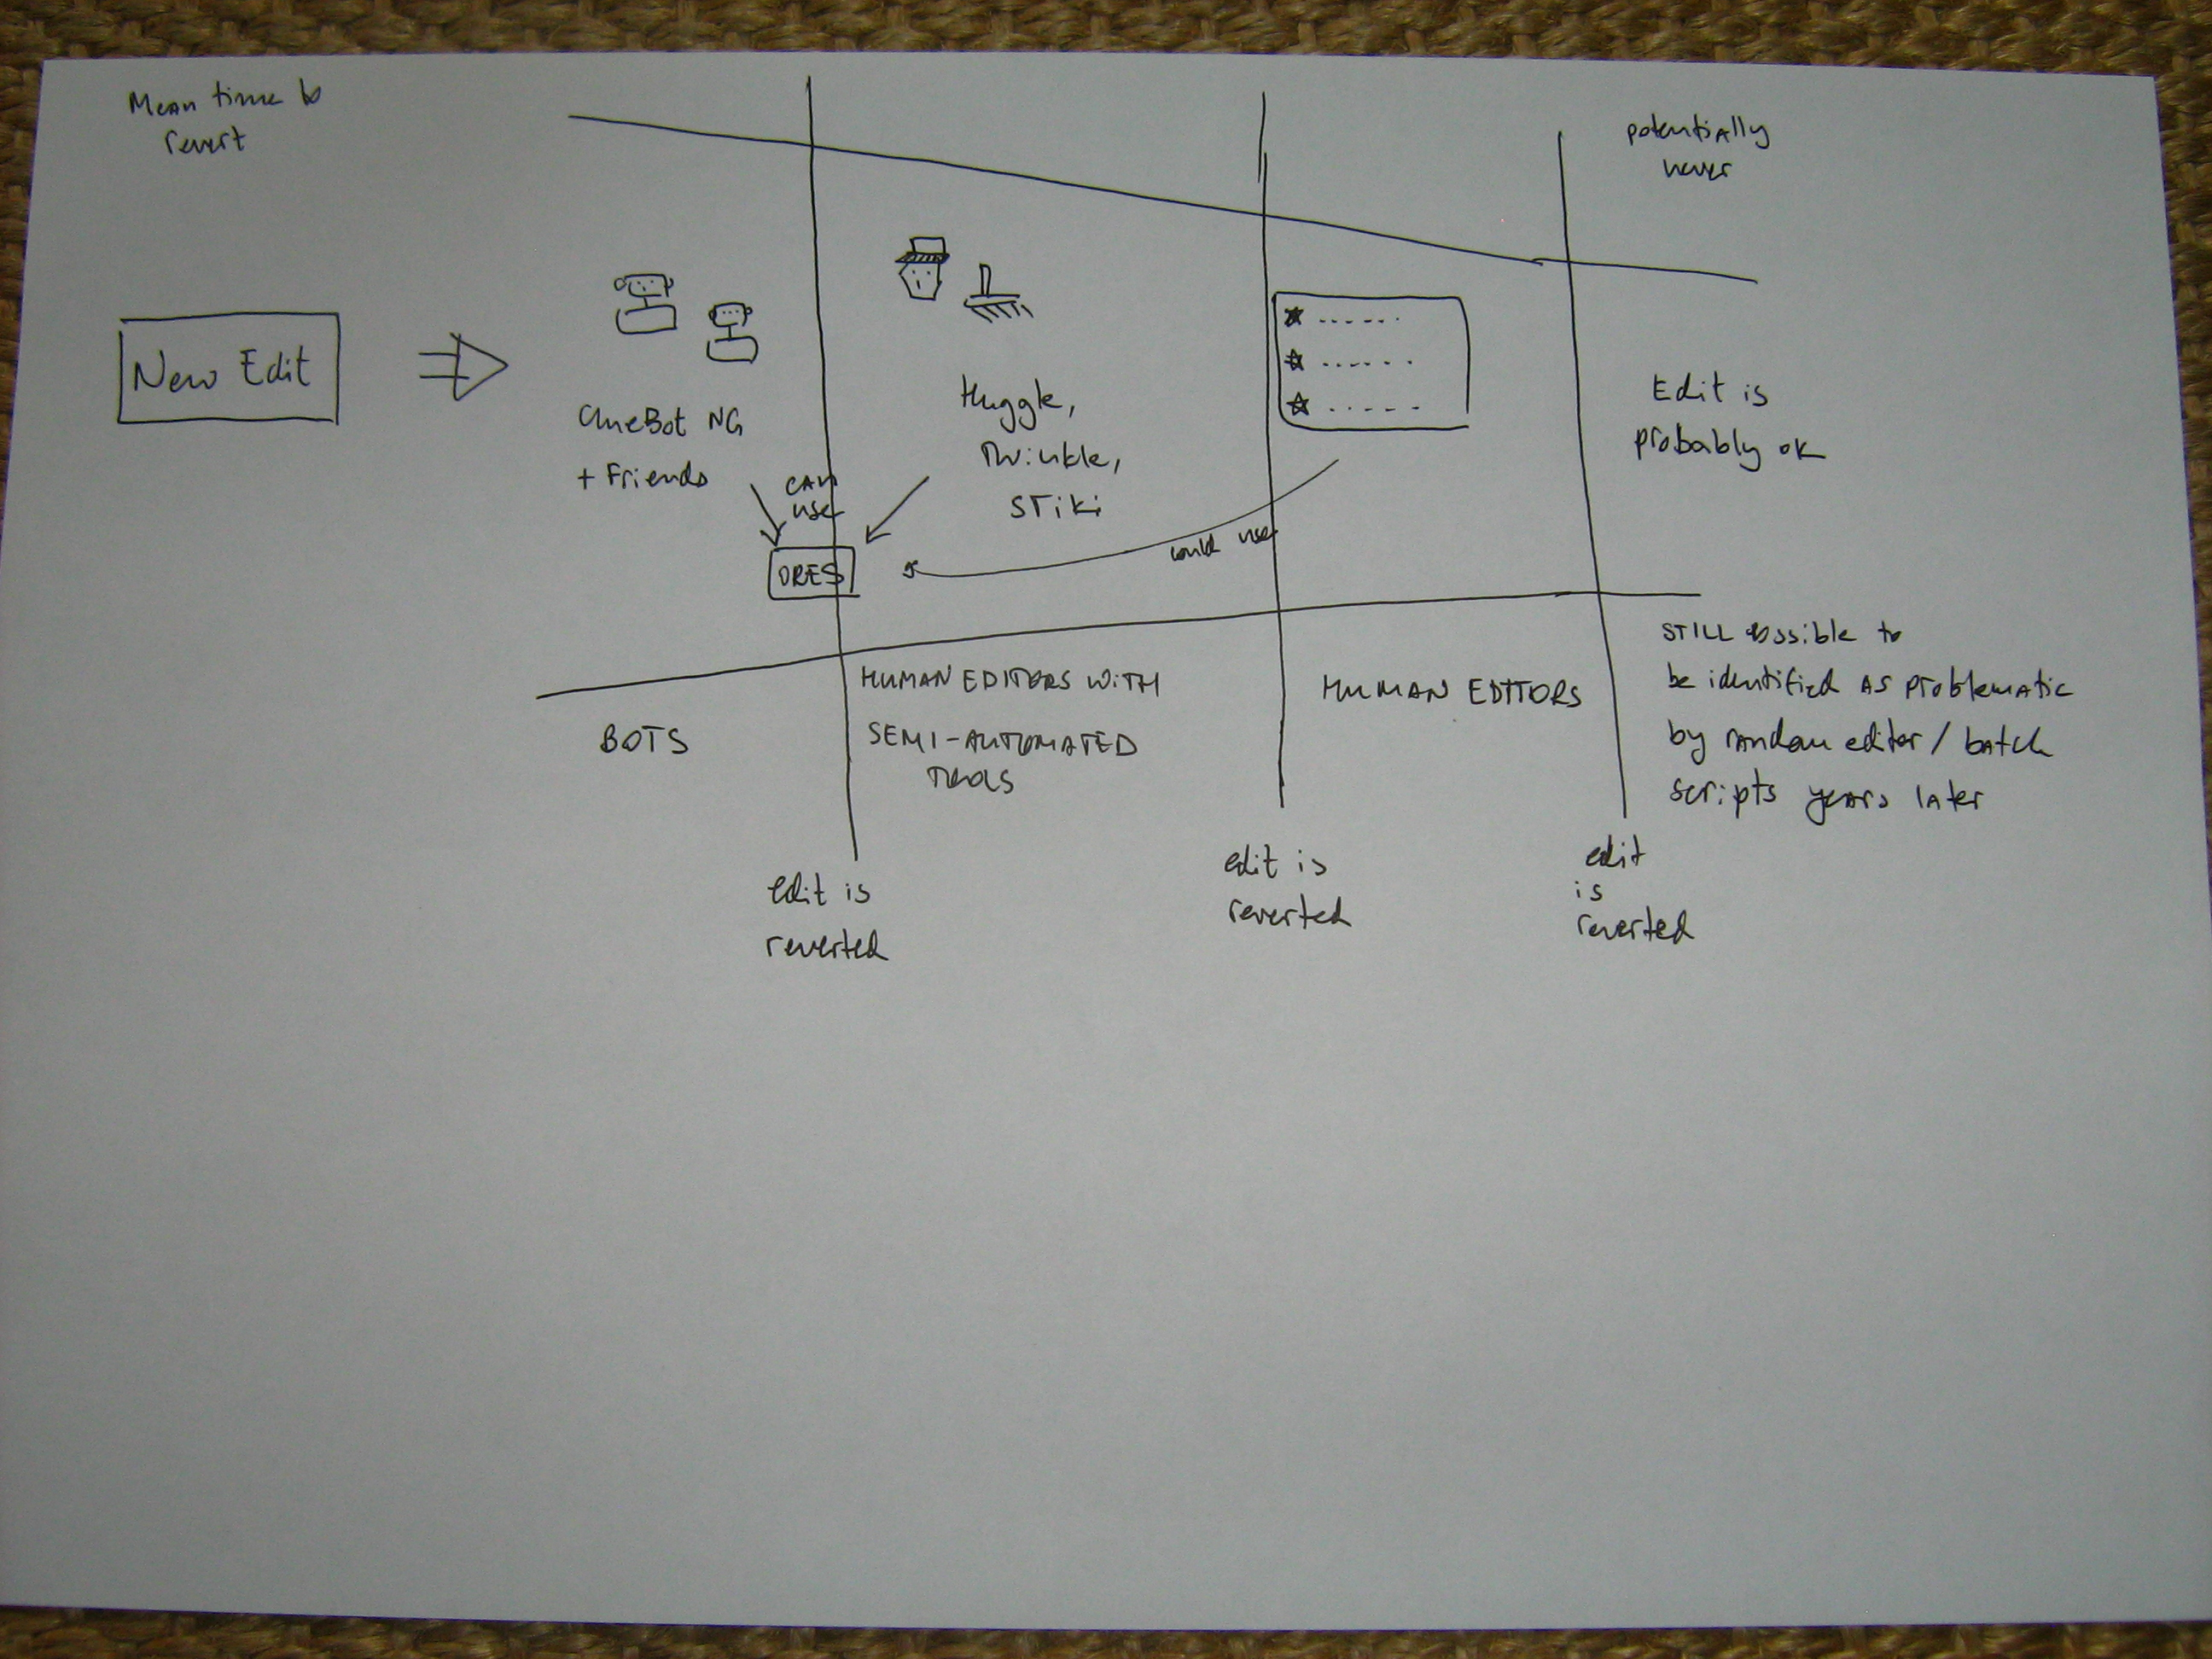
\includegraphics[width=0.9\columnwidth]{pics/funnel-diagramm-no-filters.JPG}
  \caption{State of the scientific literature: edit filters are missing from the quality control frame}~\label{fig:funnel-no-filters}
\end{figure}

%TODO check which entries actually result from the text!!
% and get rid of the empty page that follows
\begin{landscape}
    \begin{longtable}{ | p{4cm} | p{5.5cm} | p{5.5cm} | p{5.5cm} | }
    \hline
               & Bots & Semi-Automated tools & ORES \\
    \hline
    \multirow{7}{*}{Properties} & rule/ML based & rule/ML based & ML framework \\
                               & run on user's infrastructure ("bespoke code") & extra infrastructure & not used directly, can be incorporated in other tools \\
                               & no requirement for code to be public & most popular are open source (but not a hard requirement) & open source \\
                               & & heuristics obfuscated by the interface & \\
                               & latency varies & generally higher latency than bots & \\
                               & mostly single dev/operator (recently: bot frameworks) & few devs & few devs \\
    \hline
    \multirow{2}{*}{People involved} & no special rights needed (except for admin bots) & \emph{rollback} permission needed & mostly Scoring Platform team \\
                                     & bot gets a ``bot flag'' & & \\
    \hline
        \multirow{2}{*}{Hurdles to participate} & get approval from the BAG & get a \emph{rollback} permission& \\
                                            & programming knowledge, understand APIs, ... & get familiar with the tool & understand ML \\
    \hline
        \multirow{2}{*}{Concerns} & ``botophobia'' & gamification & general ML concerns: hard to understand \\
                                  & & & \\
    \hline
        Areas of application & mostly obvious vandalism & less obvious cases that require human judgement & \\
    \hline
    \caption{Wikipedia's algorithmic quality control mechanisms in comparison}~\label{table:mechanisms-comparison-literature}
\end{longtable}
\end{landscape}
